\graphicspath{{./images/chapter04/bmps/}{./images/chapter04/vects/}{./images/chapter04/}}

\chapter{Stixel World}\label{ch:chapter04}

In the previous chapter, we saw a set of algorithms and configurations able to construct a disparity map from a pair of stereo images. These methods are useful for the reconstruction of the environment. However, this reconstruction is dense, which leads to an intensive usage of the computer resources. In order to solve this problem, some authors propose approaches that try to minimize the area of the image being processed by doing a simpler reconstruction than that done with dense 3D reconstruction algorithms. In this sense, \cite{badino2009stixel} proposed to represent the world by a set of rectangular sticks named \emph{stixels} (from \emph{stick} and \emph{pixel}). Each stixel is defined by its 3D position relative to the camera and stands vertically on the ground, having a certain height.
This compact but flexible representation of the world can be used as the common basis for the scene understanding tasks of driver assistance and autonomous systems. The main advantages of using such an approach are listed next:
\begin{itemize}
 \item \emph{Compact}. Significant reduction of the data volume.
 \item \emph{Complete}. Information of interest is preserved.
 \item \emph{Stable}. Small changes of the underlying data must not cause rapid changes within the representation.
 \item \emph{Robust}. Outliers must have minimal or no impact on the resulting representation.
\end{itemize}

The method described in this chapter is based in the fast stixels implementation described in \cite{benenson2012pedestrian}. One of the main advantages of this implementation is that there is no need of obtaining a previous depth map. This fact is also the main reason for which we did not use the original implementation from \cite{badino2009stixel} or that from \cite{pfeiffer2010efficient}. Based on the output of this method, we do the tracking of the stixels following a bipartite-graph method based on a given cost metric. In this sense, we have tested several cost metrics, which are described in the following sections.

Our tracking method is based on the contribution by \cite{gunyel2012stixels}. There, movement is just computed for the areas which are covered by stixels. It has been demonstrated that stixels are good enough to do a representation of the surroundings of a vehicle, and that they have a detail level enough for the movement detection. Traditionally, this movement detection is carried out through the computation of the optical flow between two frames, which is computationally expensive. In this chapter, we will see how this movement can be computed also using the stixel world representation, by extending the method of \cite{gunyel2012stixels}. For that, we have followed two different approaches, each with its own benefits and drawbacks. The first tries to cluster the stixels in objects, so the tracking is performed at object level; the second joins the stixel tracking with the object tracking in a two level tracking scheme.

Our contribution in this work is summarized next:
\begin{enumerate}
 \item Improvement of the reconstruction obtained by the stixels. The free space computation without the use of a disparity map have some drawbacks. Some of them are related with the fact that the precision in the reconstruction of the obstacles is not good enough. The object reconstruction detection scheme proposed in this chapter allows the correction of the stixel depths and the removal of the fake obstacles, as described in sections \ref{ch:chapter04_02_01} and \ref{ch:chapter04_02_02}.
 \item Improvement of the results obtained by the method described in \cite{gunyel2012stixels}, in both object and two-level tracking approaches. We modified the method by using a graph-based approach instead of a \ac{DP} based method, as they did. 
 \item Different cost metrics for the tracking have been tested, with promising results. 
 \item Faster tracking. As we will see in section \ref{ch:chapter04_02_04}, the speed achieved with our implementation is better, specially in the object based tracking. The two-level tracking is also a little bit faster, thanks to the usage of a bipartite graph based method for the matching of the stixels between frames.
 \item Our method is slightly more robust after changes between images (for example, in presence of a low framerate), specially in the case of the just object based approach.
\end{enumerate}

In the following section, each of the steps of the method are detailed. At the end of the chapter some results are shown in order to evaluate the performance of the described method.

\section{The Method}\label{ch:chapter04_01}

The method follows a pipeline as that described in figure \ref{fig:cp04_pipeline}. First, from a given pair of images, the free space in front of the vehicle is computed in order to estimate the ground plane. From the extracted ground plane, stixels are obtained. Then, a two-level tracking approach is started. The first level is that corresponding to the tracking of the stixels. This stage is inspired by the work described in \cite{gunyel2012stixels}. The set of stixels computed for the current frame are compared with those from the previous frame. Based on this comparison, some of them are matched. At the same time, we cluster stixels based on their position once projected in the 3d world. Using the clusters and the tracked stixels, we start a new tracking step in which the tracking is performed at object level. At the end of this step, we will know the obstacles in the scene and their velocities, as well as an historic of the path followed by them that could be useful for future movement estimation.

We also propose another solution in which just the object level tracking is performed. In this case, instead of doing a comparison at stixel level, we compare each obstacle to the obstacles detected in the previous frame, so the stixel level tracking is not needed anymore. In section \ref{ch:chapter04_02}, we will see the advantages and drawbacks of using one or another approach.

\begin{figure}[h!]
  \centering
  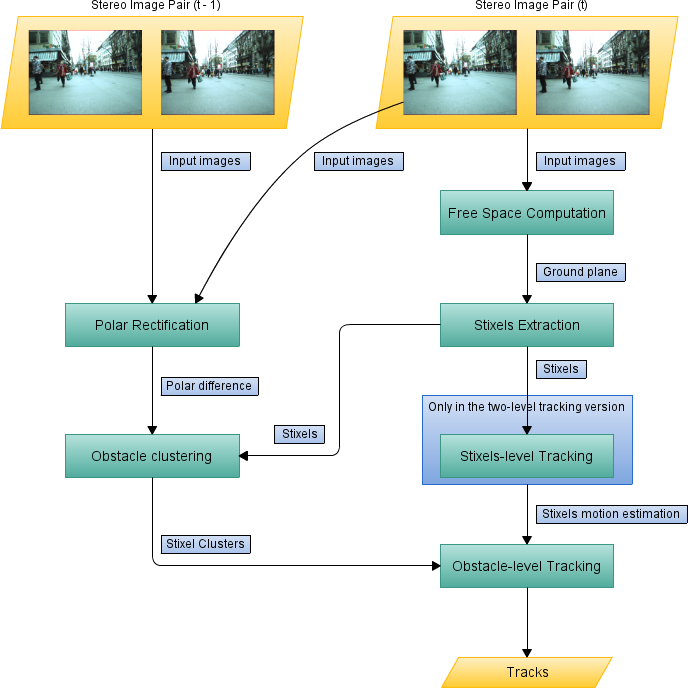
\includegraphics{pipeline}
  \caption{Pipeline of the stixels tracking method described in this chapter.}\label{fig:cp04_pipeline}
\end{figure}

\subsection{Free space computation}\label{ch:chapter04_01_01}

In this section and in the following, we will describe the stixel extraction method, which is similar to that described in \cite{benenson2012pedestrian}. This method works under the following assumptions:

\begin{itemize}
 \item The input of the algorithm is a calibrated stereo image pair.
 \item We use the Lambertian surface assumption.
 \item The ground is planar, at least at local level.
 \item The objects of interest are mainly vertical, and have a limited height range.
 \item Stereo rig has a negligible roll with respect to the ground plane.
\end{itemize}

In this section, we introduce the first step needed for the stixels estimation process, which is the ground plane estimation stage. This ground plane is estimated using the evidences collected in the \emph{v-disparity} domain. Instead of computing and projecting a depthmap obtained, for example, one of the methods evaluated in chapter \todoref{XXX}, the evidence is collected directly from matching the rows from the left and right images at different disparities, obtaining a cube $(U, V, D)$ in which each cell represents the cost of matching the pixel at $p_i(u_i, v_i) \in I_L$ with that at $q_i(u_i + d_i, v_i) \in I_R$. Here, $p_i$ and $q_i$ are pixels from the left ($I_L$) and right ($I_R$) images, respectively; and $u_i$, $v_i$ and $d_i$ are the different possible column, row and disparity values in the cube. In figure \ref{fig:cp04_freespace}, a graphical description of the obtained cube is represented.

\begin{figure}[h!]
  \centering
  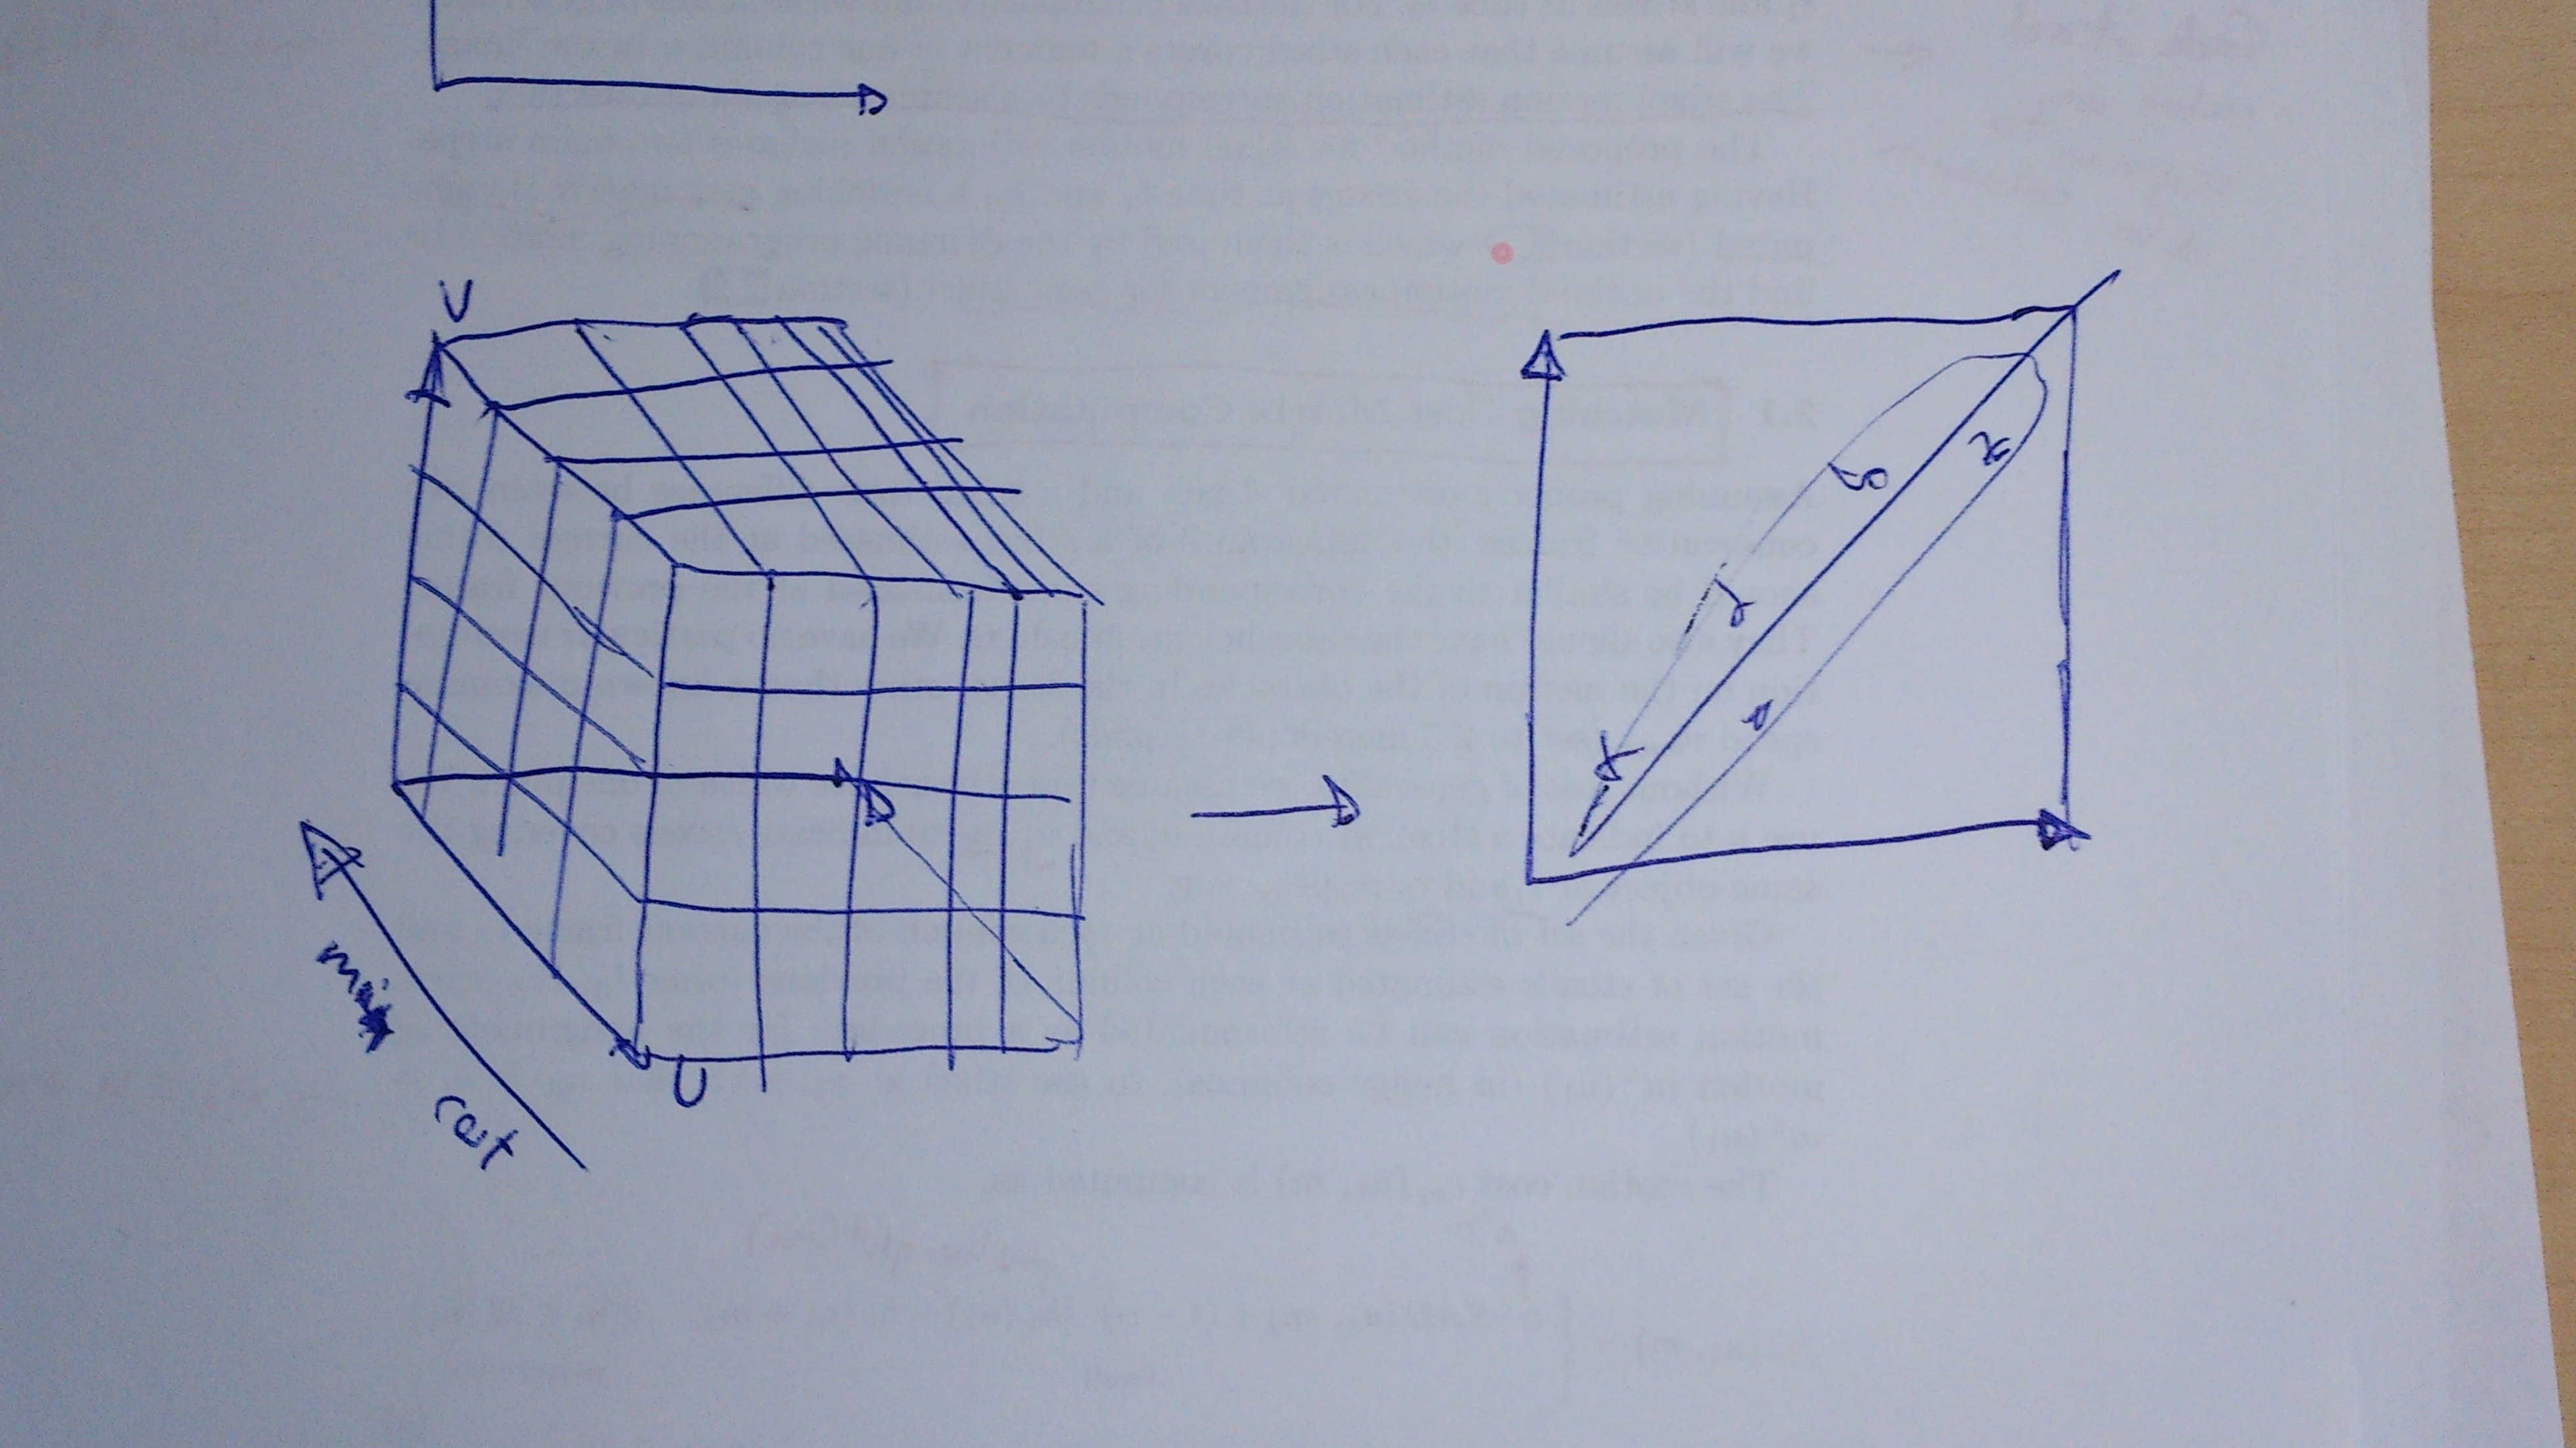
\includegraphics{freespace}
  \caption{Free space computation process.}\label{fig:cp04_freespace}
\end{figure}

For each row $v_i$, the disparity with the lowest cost is extracted for each row, as depicted in figure \ref{XXX}. From these values, a robust line fitting is used in order to find the ground plane, which is represented by the following expression:

\begin{equation}\label{eq:cp04_ground_plane_function}
  d_i = f_{ground}(v_i)
\end{equation}

Using this equation, we can know the disparity associated to each row at ground level, which will we use later for the stixels computation. For optimization purposes, instead of collecting the evidences for each row below the horizon, just one out of each $N$ rows is computed. 

\subsection{Stixels extraction}\label{ch:chapter04_01_02}

With the ground plane, we can start detecting the stixels in the images. The way in which this is done is by dividing the image in multiple row bands $b_i$. Inside each band $b_i$, and for each column $u_i$, the pixel with the biggest horizontal gradient is selected. This reduces the computational cost while the possibilities of finding the border of the object accurately are increased. Also, one of the advantages of using bands and not the rows directly is that, in presence of a confusing horizontal line, the effect is compensated by the band height.

From \ref{fig:cp04_freespace}, we obtain:

\begin{equation}\label{eq:cp04_ground_plane_function_by_band}
  d(q_j, b_i) = f_{ground}(v(q_j, b_i))
\end{equation}

Here, $q_j$ makes reference to the stixel $j$, where the total number of stixels is the total number of columns in the image divided by a parameterized stixel width $\tau_{stixel\_width}$. That is, $j=1 \dots \tau_{stixel\_width}$. In general, interest objects are wider than one column, so computing an evidence for each column in the image is redundant. Each stixel is located in the column $u(q_j) = j \cdot \tau_{stixel\_width}$. $v(q_j, b_i)$ is a certain row inside the stixel $q_j$ in the band $b_i$. 

At this point, the goal is to localize the optimal band for each stixel. This is based on the following expression:

\begin{equation}\label{eq:cp04_stixel_band_cost}
  b^*_s (q) = \underset{b(q)}{\arg\min} \underset{q}{\sum}c_s(q, b(q)) + \underset{q_a, q_b}{\sum}s_s(v(q_a, b(q_a)), v(q_b, b(q_b)))
\end{equation}

Here, we can think on $c_s$ as the data term, while $s_s$ is the smooth term. $q_a$ and $q_b$ are neighbors. That is, $|q_a - q_b| = 1$

\paragraph{Data term}\label{ch:chapter04_01_02_01}

By computing the cost $c_s$, we know the likelihood of the presence of an stixel $q$ at the row band $b$. The lower the cost is, the more possible that there is a stixel. This cost is computed as follows:

\begin{equation}\label{eq:cp04_stixel_band_cost_data_term}
  c_s(q, b) = c_o (u(q), d(q, b)) + c_g(u(q), d(q,b))
\end{equation}

This equation is composed by two terms:
\begin{itemize}
 \item \emph{Object cost($c_o$)}. It represents the cost of the presence of a vertical object. It just sums the evidence along the vertical column, using the expected height of the object, which is projected on the image using the distance given by the ground plane.
 \item \emph{Ground cost($c_g$)}. It represents the cost of a supporting ground being present, and sums the evidence along the ground plane.
\end{itemize}

\paragraph{Smooth term}\label{ch:chapter04_01_02_02}

The smooth term ($s_s$) forces to respect the left-right occlusion restrictions and promotes ground object boundaries with few jumps.

\begin{equation}\label{eq:cp04_stixel_band_cost_smooth_term}
  s_s(v_a, v_b) = 
  \begin{align*}
    \begin{cases}
    \infty & \text{if } d(v_a) < d(v_b) - 1 \\
    c_o(u_a, d(v_a)) & \text{if } d(v_a) \approx d(v_b) - 1 \\
    - \omega \cdot c_o(u_a, d(v_a)) & \text{if } q_a = q_b \\
    0 & \text{if } d(v_a) > d(v_b) - 1
    \end{cases}
  \end{align*}
\end{equation}

Here, $\omega$ is a free parameter, chosen by the user, which promotes boundaries with a few jumps. At this point, we will have extracted the stixels, obtaining a result similar to that shown at figure \ref{fig:cp04_stixels}, in which the stixels (in green) are superimposed to the left image from which they were extracted. For more information about the process described in sections \ref{ch:chapter04_01_01} and \ref{ch:chapter04_01_02}, please refer to \cite{benenson2012fast}.

\begin{figure}[h!]
  \centering
  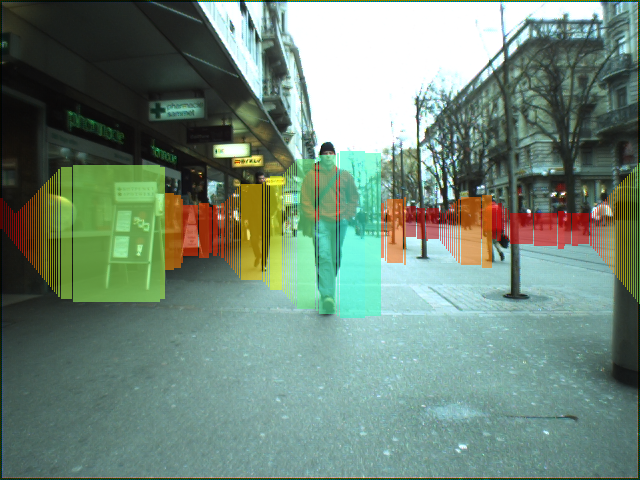
\includegraphics{stixels_over_original}
  \caption{Stixels superimposed to the frame from which they were extracted.}\label{fig:cp04_stixels}
\end{figure}

\subsection{Tracking}\label{ch:chapter04_01_03}

At this point, we are ready to start tracking the stixels. As said before this tracking has been performed using two different approaches: one consists on two different tracking levels from the first one tracks the stixels independently (that is, each stixel at the previous frame $t - 1$ is matched with another - or none - at the current frame $t$). So it becomes a matching problem in which we try to find the minimal cost matching between frames. In \cite{gunyel2012stixels}, this minimal matching was done using \ac{DP}. In our implementation we use a bipartite graph matching based method. In a second level, stixels are clustered into objects, which are matched based on the previous stixels tracking.

In the other approach, just the second level is performed, tracking obstacles based on one of the cost metrics, without considering the stixels included in the objects (except for the clustering process). In the next sections, the tracking process is described. Please note that the process described in section \ref{ch:chapter04_01_03_01} is performed only for the two-level approach, while the process in \label{ch:chapter04_01_04} is common to both approaches, except from the differences explicitly indicated in that section.

For this stage, we made some assumptions:
\begin{itemize}
 \item First, we assume that all stixels have been properly estimated.
 \item The maximal speed of the objects is limited, so we limit the search range between stixels to a certain threshold. This range depends on the distance of the stixel at the current frame and the frame rate. As there is just one stixel per column, we can limit also the matching process to a search into the $u$ direction.
 \item There is not a big temporal difference between two consecutive frames. That means that the same stixel at time $t$ and $t - 1$ should be similar. Also their height in meters should be similar. \notsure{As shown in section \ref{ch:chapter04_02_03_02}, this temporary consistence is more or less restrictive depending on the approach finally used for the tracking process.}
\end{itemize}

\subsubsection{Stixels-level tracking}\label{ch:chapter04_01_03_01}

In this stage, the tracking is performed at stixel level. As we just try to match each stixel at column $q_i\{t\}$ with another in the previous frame $t - 1$, we can think on this process as a matching problem. The way in which we have solved this is through a bipartite graph, in which nodes are the stixels at frame $t$ and $t - 1$, and the edges are associated to a certain movement cost $c_m$, which is represented by the equation:

\begin{equation}\label{eq:cp04_stixel_movement_cost}
  c_m(u_i\{t\}, u_j\{t - 1\}) = 
  \begin{align*}
    \begin{cases}
    f_{cost}(u_i\{t\}, u_j\{t - 1\}) & \textbf{if} \text{ matching is applicable} \\
    \infty & \textbf{otherwise}
    \end{cases}
  \end{align*}
\end{equation}

Here, a matching is applicable if and only if the following restrictions are satisfied:
\begin{itemize}
 \item $|X(u_i\{t\}) - X(u_j\{t - 1\})| < \tau_{max\_disp}$, where the free parameter $\tau_{max\_disp}$ indicates the maximal displacement of a certain stixel between frames; and $X(u)$ refers to its $X$ position in 3d coordinates.
 \item $u_i\{t\}$ is not a new stixel. That is, this is not the very first frame in which the stixel appears.
 \item Stixels $u_i\{t\}$ and $u_j\{t - 1\}$ are not occluded.
 \item $f_{cost}(u_i\{t\}, u_j\{t - 1\}) < \tau_{max\_cost}$.
\end{itemize}

Else, the cost is considered as infinity, so the link is not included in the graph. $f_{cost}(u_i\{t\}, u_j\{t - 1\})$ is a cost function which can be composed by different cost metrics, weighted by a set of parameters in the form:

\begin{equation}\label{eq:cp04_cost_function}
\small
  \begin{align*}
  f_{cost}(u_i\{t\}, u_j\{t - 1\}) =~  & & \alpha_{SAD} & ~\cdot~ & f_{SAD}(u_i\{t\}, u_j\{t - 1\}) \\
      & + & \alpha_{hist} & ~\cdot~ & f_{hist}(u_i\{t\}, u_j\{t - 1\}) \\
      & + & \alpha_{height} & ~\cdot~ & f_{height}(u_i\{t\}, u_j\{t - 1\})
  \end{align*}
\end{equation}

Here, $\alpha_{SAD} + \alpha_{hist} + \alpha_{height} = 1$. $f_{SAD}(u_i\{t\}, u_j\{t - 1\})$, $f_{hist}(u_i\{t\}, u_j\{t - 1\})$ and $f_{height}(u_i\{t\}, u_j\{t - 1\})$ are the factors for the different cost metrics being tested, which are described next.

\subsubsection{\acf{SAD}}\label{ch:chapter04_01_03_01_01}

This cost is computed as the pixel-wise sum of the absolute differences over the RGB color scheme between $u_i\{t\}$ and $u_j\{t - 1\}$, following the expression

\begin{equation}\label{eq:cp04_stixel_movement_sad_cost}
\tiny
f_{SAD}(u_i\{t\}, u_j\{t - 1\}) = 
\overset{v_b(q_i\{t\})}{\underset{v_1=v_a(q_i\{t\})}{\sum}}
\overset{v_b(q_j\{t - 1\})}{\underset{v_2=v_a(q_i\{t - 1\})}{\sum}}
| I_L\{t\}(u_i\{t\}, v_1) - I_L\{t - 1\}(u_j\{t - 1\}, v_2) |
\end{equation}

As it is very unlikely for both stixels to have the exact same height, they are resized to a dimension of $30\,px$. This metric was originally used in \cite{gunyel2012stixels} for the computation of the movement of the stixels. It has been used in our tests to compare the our results with those obtained by them in their implementation.

\subsubsection{Histograms matching}\label{ch:chapter04_01_03_01_02}

As said, the same stixel has not always the same size in different frames. This can happen because the position of the object partially represented by the stixel can change its depth in the scene, or due to noise in the height detection of the stixel. In order to normalize this, we have computed the histogram of each of the stixels being compared. Then, the cost is computed from the Hellinger distance between both histograms:

\begin{equation}\label{eq:cp04_stixel_movement_histograms_cost}
f_{SAD}(u_i\{t\}, u_j\{t - 1\}) = 2 \cdot \sqrt { 1 - \underset{i=1}{\overset{d}{\sum}}\sqrt{H(u_i\{t\})[i] \cdot H(u_j\{t - 1\})[i]}}
\end{equation}

Here, $H(u)[i]$ is the $i^{th}$ bin of the histogram computed for the stixel $u$, and $d$ is the number of bins in the histogram. In our implementation, $d = 256$.

\subsubsection{Height difference}\label{ch:chapter04_01_03_01_05}

This metric is used to complement the other two metrics, as by its own is not enough to do a matching, but it is good enough to help in the decision, in case of very similar scores in two or more possible matches. $f_{height}$ is computed as follows:

\begin{equation}\label{eq:cp04_stixel_movement_height_cost}
f_{height}(u_i\{t\}, u_j\{t - 1\}) = 1 - |h(u_i\{t\} - h(u_j\{t - 1\})|
\end{equation}

, where $h(u)$ is the height of the stixel in column $u$. 

In our tests, we have tried different values for $\alpha_{SAD}$, $\alpha_{hist}$ and $\alpha_{height}$, obtaining the results shown in section \ref{ch:chapter04_02}, both in terms of performance and time. As said, the value obtained using the function $f_{cost}$ is used to weight the links between the nodes of a bipartite graph. This graph, whose nodes are the stixels at times $t$ and $t - 1$, is shown at figure \ref{fig:cp04_bipartite_graph}. In the top row, we can see the nodes (stixels) at current time, while in the lower row, previous stixels are represented. Costs of the match are represented by the edges, depicted in the image with the notation $\omega_{i,j}$.

\begin{figure}[h!]
\centering
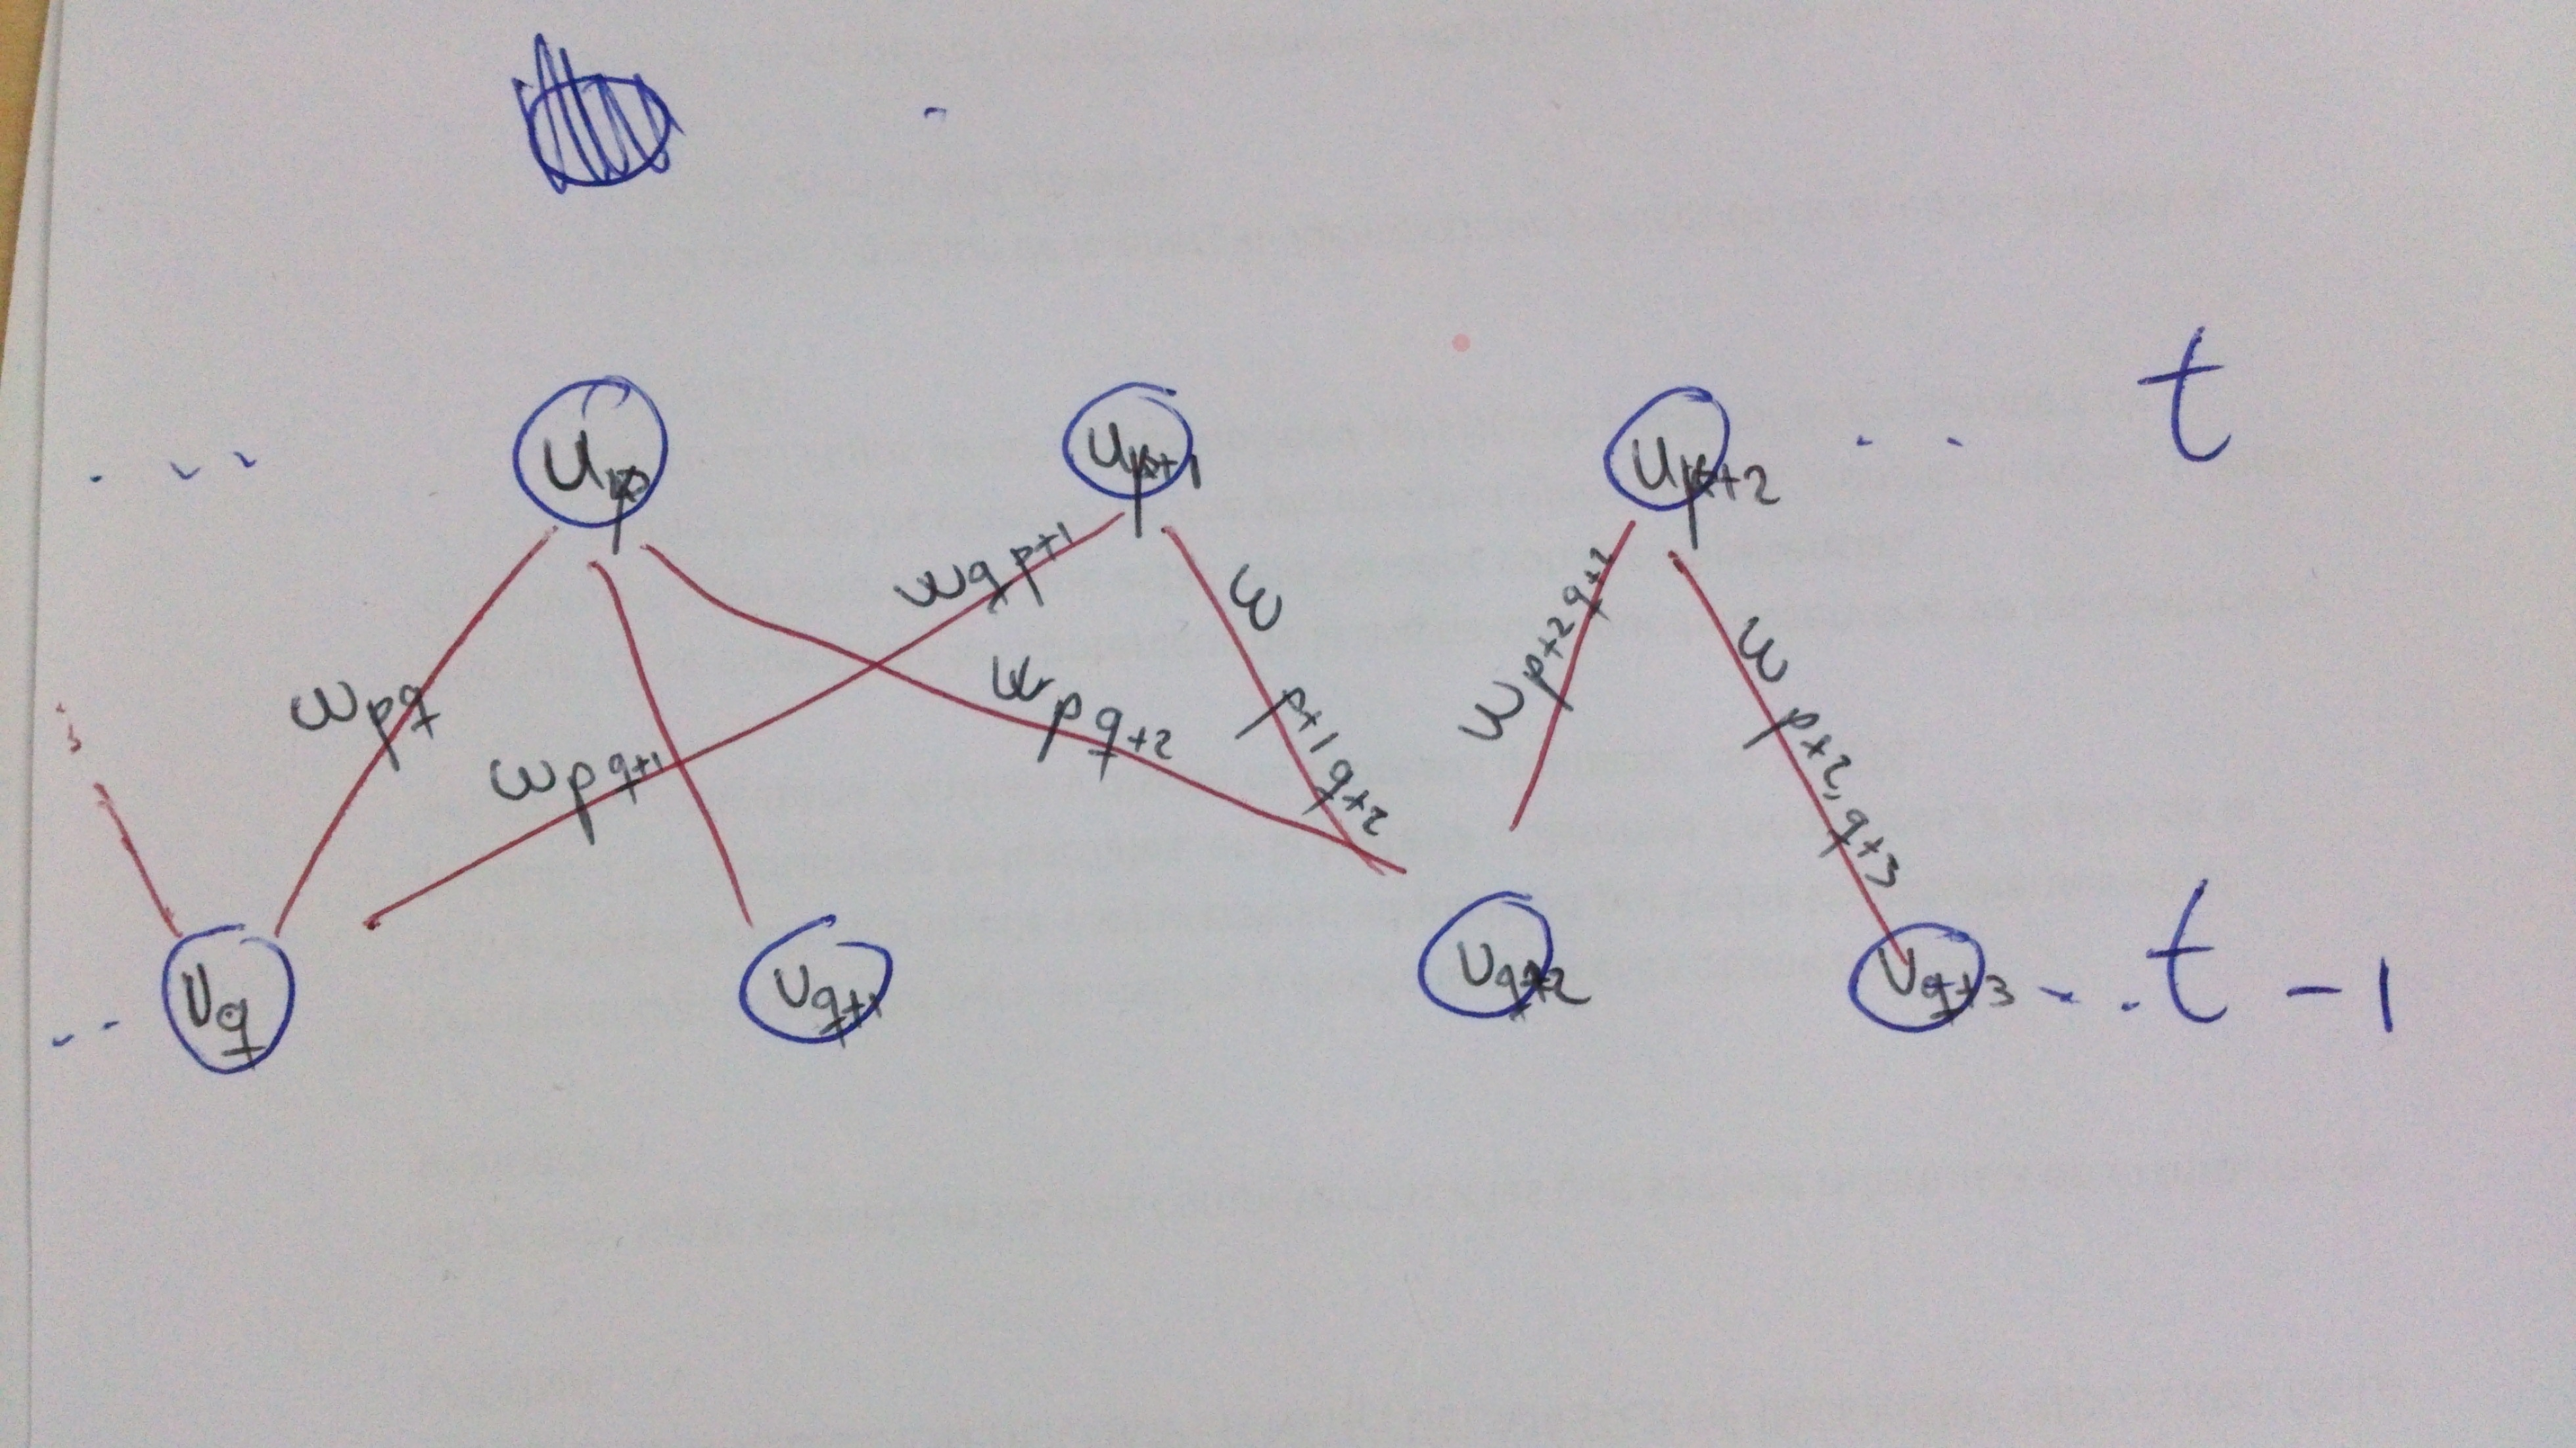
\includegraphics{bipartite_graph}
\caption{Representation of the bipartite graph used for the matching process.}\label{fig:cp04_bipartite_graph}
\end{figure}

Over this graph, we solve the following minimization problem:

\comment{No estoy seguro de esta notación}
\begin{equation}\label{eq:cp04_match_minimization}
\mathcal{\hat{M}}=\underset{\mathcal{M}}{\arg\min} \underset{(i, j) \in \mathcal{M}}{\sum} \omega_{i,j}, 
~~~~\exists! (i, \cdot) \wedge \exists! (\cdot, j)
\end{equation}

This problem is solved using a $O(n \cdot m \cdot log(n))$ implementation of the Edmond's maximum weighted matching algorithm (\cite{edmonds1965paths}). The advantages of using this method instead the \ac{DP} implementation by \cite{gunyel2012stixels} is that we getter better times that the implementation available and, specially, we can ensure that each match is performed one-to-one. That is, in the \cite{gunyel2012stixels} implementation, the same stixel could be matched with more than one stixel from the other frame. This is not good, as we can have multiple paths from the same stixel, so it is difficult to know the trajectory it has followed in the past. In our implementation, we choose the matching set that maximizes the whole matching, ensuring that one stixel is matched with \emph{only} one stixel in the other frame.

\subsection{Obstacle-level tracking}\label{ch:chapter04_01_04}

In this stage, we perform the tracking at obstacle level, and not at stixel level, as described in the previous section. In the case of two-level tracking, we should have at this point the set of matchings $m(i,j) \in \mathcal{M}$, which relates each stixel at column $u_i$ in the frame $t$ with the stixel at column $u_j$ in the frame $t - 1$. Anyway, we do not really need to have these matches for this stage, and do the tracking directly at the obstacle level. This section comprises two steps: object detection (clustering) and object tracking.

\subsubsection{Clustering}\label{ch:chapter04_01_04_01}

From left to right, stixels are being evaluated using the algorithm shown at algorithm \ref{alg:cp04_clustering}.

\begin{algorithm}
\caption{Clustering algorithm}
\label{alg:cp04_clustering}
\begin{algorithmic}
\Function{Clustering}{$\mathcal{Q}\{t\}$}
  \State {$\mathcal{O} \gets \emptyset$}
  \State {$o \gets \emptyset$}
  \For {\textbf{each} stixel $q_i \in \mathcal{Q}$, from left to right}
    \If {$|depth(q_i) - depth(q_{i-1})| > \tau_{depth\_dist}$}
      \If {$|depth(q_i) - depth(q_{i-1})| > \tau_{depth\_dist}$}
	\State {$width(o) > \tau_{min\_width}$}
      \EndIf
      \State {$o \gets \emptyset$}
    \EndIf
    \State {$o \gets o \cup q_i$}
  \EndFor
\EndFunction
\end{algorithmic}
\end{algorithm}

There, $\mathcal{Q}\{t\}$ is the set of stixels for the current frame $t$. From left to right, we start accumulating stixels, until the difference in depth between a certain pair of stixels is above a threshold $\tau_{depth\_dist}$, which is a user-defined free parameter. When this difference appears, we consider that we reached the right border of the obstacle, so it is added to the set $\mathcal{O}$, and a new obstacle is started. In case an obstacle is not wide enough, this obstacle is rejected. The reason for that is there are a stixel for each column, so there is a lot of noise that must be removed. This effect is easy to notice if we look at figure \ref{fig:cp04_stixels}.

At the end of the process, we will have got the set of obstacles $o_i \in \mathcal{O}$. Each obstacle has associated several parameters. One of them is the depth, which is computed as the minimal depth of all the associated stixels. In the left image of figure \ref{fig:cp04_clustering_aggregation}, the output obtained once this process has finished is shown.

\paragraph{Obstacle aggregation}\label{ch:chapter04_01_04_01_01}

In certain cases, due to a bad stixel detection, some stixels are located wrongly at a different depth from their real position. This effect happens, for example in cases like that shown at the left image of figure \ref{fig:cp04_clustering_aggregation}, in which a person in a fist plane opens his legs wide enough to show a big portion of the ground which is after him. This confuses the stixels detection algorithm, which thinks that the base of the obstacle is the central part of this person, and not his feet.

To solve this problem, the process described in algorithm \ref{alg:cp04_aggregation} is performed.

\begin{algorithm}
\caption{Aggregation algorithm}
\label{alg:cp04_aggregation}
\begin{algorithmic}
\Function{Aggregation}{$\mathcal{O}$}
  \State {$\mathcal{O'} \gets \emptyset$}
  \State {$o' \gets \emptyset$}
  \For {\textbf{each} object $o_i \in \mathcal{O}$, from left to right}
    \If {$|X(o_i) - X(o_{i-1})| > \tau_{lateral\_aggregation\_dist}$ \textbf{or}\\ \indent\indent\indent
	 $|Z(o_i) - Z(o_{i-1})| > \tau_{depth\_dist}$ \indent\indent~}

      \State {$\mathcal{O} \gets \mathcal{O} \cup o'$}
      \State {$o' \gets \emptyset$}
    \EndIf
    \State {$o' \gets o' \cup o$}
  \EndFor
\EndFunction
\end{algorithmic}
\end{algorithm}

There, we test all obstacles previously detected, again from left to right. If the lateral distance (in world coordinates) is below a threshold $\tau_{lateral\_aggregation\_dist}$, we check again if the depth difference is below $\tau_{depth\_dist}$. If this condition is satisfied, both obstacles are joined together. In figure \ref{fig:cp04_clustering_aggregation}, an example of the output obtained from this process is shown. In the left image, the person in the first plane is divided into two different obstacles. After the aggregation process, this same person is assigned to a single obstacle. Depth of the obstacle is computed as the minimal depth of both original obstacles.

\begin{figure}[h!]
\begin{tabular}{cc}
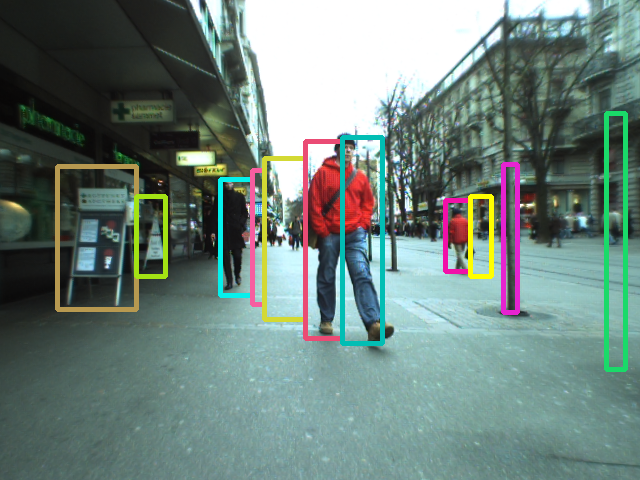
\includegraphics[width=0.49\textwidth]{obstaclesBeforeAggregation}\label{fig:cp04_before_aggregation} &
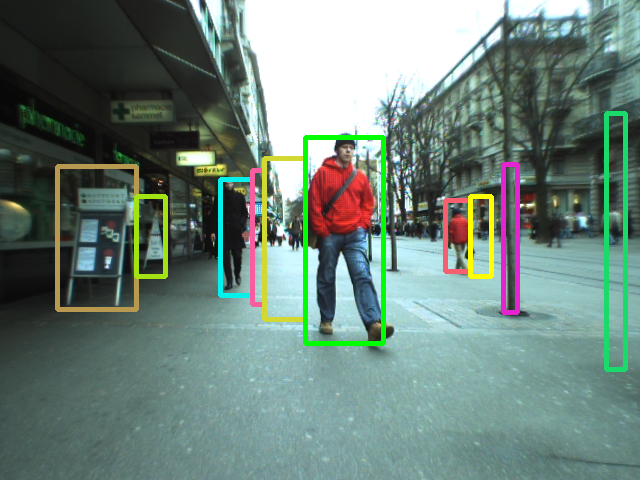
\includegraphics[width=0.49\textwidth]{obstaclesAggregated}\label{fig:cp04_after_aggregation}
\end{tabular}
\caption{Comparison of the obstacles detected before and after the aggregation process.}\label{fig:cp04_clustering_aggregation}
\end{figure}

\paragraph{Obstacle filtering}\label{ch:chapter04_01_04_01_02}

If we look again at figure \ref{fig:cp04_clustering_aggregation}, we will notice that we are still detecting some fake obstacles. For instance, between the man with the red jacket and that with the dark suit, there are two of them. Next to the man in the second plane, also with a red jacket, there is another fake obstacle, and there is a last one in the right side of the image. Signs and poles are not considered fake obstacles, as they are elements to avoid, and we do not have a classification scheme able to distinguish the class of the obstacle being detected.

In order to distinguish real obstacles from fake obstacles, we register the images obtained between frames, so we can distinguish the movement between frames. This movement can be originated both by the movement of the obstacle itself (i.e. a person walking), or by the movement of the camera respect to the obstacles. This makes occluded areas to appear, which allows detecting the border of obstacles that are not moving, but which we want to avoid. This is the case, for example, of the pole in the right part of the image.

The best way to do such a registration is through a polar rectification process, described at appendix \ref{ch:appendix_polar_calib}. With it, we will be able to align the current frame at time $t$ with another frame at time $t - k$. Using the aligned images, we get the pixel-wise absolute difference of both images, so we can get those pixels for which there is movement. This difference image is projected back to coordinates of the current image. Then, this difference is thresholded and binarized, rejecting the small differences produced by noise. Result of this process is shown at the top of figure \ref{fig:cp04_obstacle_filtering}. Then, for each obstacle, we get the associated \ac{ROI}. For each \ac{ROI}, we reject the top half of it, so we just look for movement in the area of the obstacle that is touching the ground. There are two reasons for that: the first one is that obstacles that move over the ground tend to have a higher movement in the lower part (for instance, legs or wheel movements). In the case of first plane static obstacles, the movement due to the camera change is more or less similar in the upper and lower half, so we are not loosing information. The second reason is that the stixels reconstruction assumes a planar ground in front of the camera, it is a fast way to discriminate bad correspondences.

\begin{figure}[h!]
  \begin{minipage}{\textwidth}
    \centering
    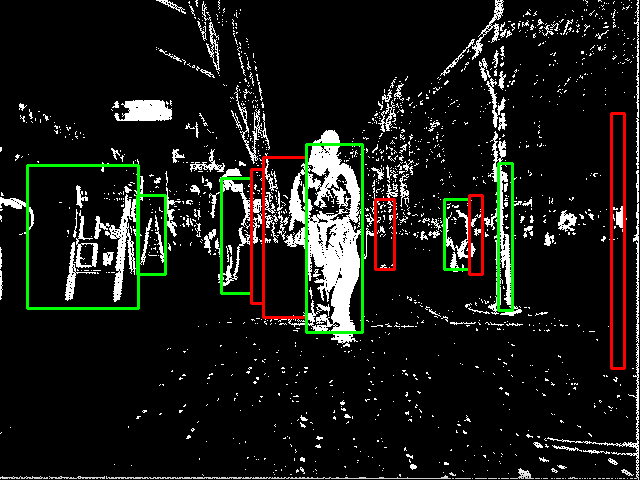
\includegraphics[width=\textwidth]{thresholdedPolar}
    \end{minipage}\hfill~
  \begin{minipage}{\textwidth}
    \centering
    \begin{tabular}{ |c|c|c|c|c|c|c|c|c|c|c|}
      \hline
      0 & 1 & 2 & 3 & 4 & 5 & 6 & 7 & 8 & 9 & 10 \\
      \hline
      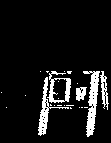
\includegraphics[width=0.15\textwidth, height=0.15\textwidth]{obstacleFilter/roi0} &
      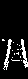
\includegraphics[width=0.15\textwidth, height=0.15\textwidth]{obstacleFilter/roi1} &
      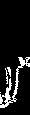
\includegraphics[width=0.15\textwidth, height=0.15\textwidth]{obstacleFilter/roi2} &
      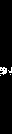
\includegraphics[width=0.15\textwidth, height=0.15\textwidth]{obstacleFilter/roi3} &
      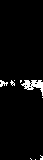
\includegraphics[width=0.15\textwidth, height=0.15\textwidth]{obstacleFilter/roi4} & 
      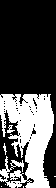
\includegraphics[width=0.15\textwidth, height=0.15\textwidth]{obstacleFilter/roi5} &
      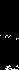
\includegraphics[width=0.15\textwidth, height=0.15\textwidth]{obstacleFilter/roi6} &
      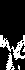
\includegraphics[width=0.15\textwidth, height=0.15\textwidth]{obstacleFilter/roi7} &
      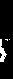
\includegraphics[width=0.15\textwidth, height=0.15\textwidth]{obstacleFilter/roi8} &
      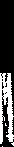
\includegraphics[width=0.15\textwidth, height=0.15\textwidth]{obstacleFilter/roi9} &
      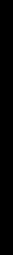
\includegraphics[width=0.15\textwidth, height=0.15\textwidth]{obstacleFilter/roi10} \\
      \hline
      \setlength{\fboxsep}{1pt}\fcolorbox{green}{green}{
\includegraphics[width=0.15\textwidth, height=0.15\textwidth]{obstacleFilter/occ0}} &
      \setlength{\fboxsep}{1pt}\fcolorbox{green}{green}{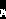
\includegraphics[width=0.15\textwidth, height=0.15\textwidth]{obstacleFilter/occ1}} &
      \setlength{\fboxsep}{1pt}\fcolorbox{green}{green}{
\includegraphics[width=0.15\textwidth, height=0.15\textwidth]{obstacleFilter/occ2}} &
      \setlength{\fboxsep}{1pt}\fcolorbox{red}{red}{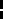
\includegraphics[width=0.15\textwidth, height=0.15\textwidth]{obstacleFilter/occ3}} &
      \setlength{\fboxsep}{1pt}\fcolorbox{red}{red}{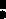
\includegraphics[width=0.15\textwidth, height=0.15\textwidth]{obstacleFilter/occ4}} & 
      \setlength{\fboxsep}{1pt}\fcolorbox{green}{green}{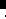
\includegraphics[width=0.15\textwidth, height=0.15\textwidth]{obstacleFilter/occ5}} &
      \setlength{\fboxsep}{1pt}\fcolorbox{red}{red}{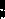
\includegraphics[width=0.15\textwidth, height=0.15\textwidth]{obstacleFilter/occ6}} &
      \setlength{\fboxsep}{1pt}\fcolorbox{green}{green}{
\includegraphics[width=0.15\textwidth, height=0.15\textwidth]{obstacleFilter/occ7}} &
      \setlength{\fboxsep}{1pt}\fcolorbox{red}{red}{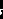
\includegraphics[width=0.15\textwidth, height=0.15\textwidth]{obstacleFilter/occ8}} &
      \setlength{\fboxsep}{1pt}\fcolorbox{green}{green}{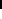
\includegraphics[width=0.15\textwidth, height=0.15\textwidth]{obstacleFilter/occ9}} &
      \setlength{\fboxsep}{1pt}\fcolorbox{red}{red}{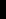
\includegraphics[width=0.15\textwidth, height=0.15\textwidth]{obstacleFilter/occ10}} \\
      \hline
    \end{tabular}
  \end{minipage}\hfill
  \caption{Object filtering process. In the top, the binarized motion image is shown ($k=0.2$). In the bottom, the occupancy maps generated for each candidate obstacle.}\label{fig:cp04_obstacle_filtering}
\end{figure}

Each region is transformed to real world coordinates and project there the points resulting after the thresholding process. There, the region is dividided in cells (in our tests, of $10\times10\,cm$). For each cell, if there is at least one point falling inside it in the plane $XY$, the cell is marked as occupied. The occupancy grids obtained, together with their associated \ac{ROI} in the motion image, are shown in the table in figure \ref{fig:cp04_obstacle_filtering}. \acs{ROI} are in the first row, and occupancy maps in the second. It is easy to see that real obstacles, like for example number 5 or number 7, present a higher density if compared with, for example, the obstacle number 4. Also, if we look at obstacle 2, a man in a black suit (which makes the motion detection a little bit more complicated through absolute differencing due to the low color values), is properly detected. In order to ensure the detection of this kind of obstacles, it is important to choose a value for $k$ big enough. In our tests, we decided to use $k = 0.2\,s$, so we are sure that differences are appreciable, but being conservative at the same time. At the end of the process, we decide if the obstacle is rejected or not through the following equation:

\begin{equation}\label{eq:cp04_fake_obstacles}
  fake(o) = 
  \begin{align*}
    \begin{cases}
      true & \text{if } {{count(G_o, true)} \over {count(G_o, true) + count(G_o, false)}} > \tau_{occ} \\
      false & otherwise
    \end{cases}
  \end{align*}
\end{equation}

There, $count(G_o, j)$ counts the number of occupied ($j=true$) or free ($j=false$) cells in the occupancy grid corresponding to the object $o$, $G_o$. $\tau_{occ}$ is a parameter. We also check that the width of each obstacle in real world coordinates is inside the limits. We can see the results obtained for this process again in figure \ref{fig:cp04_obstacle_filtering}. Rejected obstacles are highlighted in red, while the accepted are represented in green.

\subsubsection{Tracking}\label{ch:chapter04_01_04_02}

Once we have the obstacles detected and filtered, we propose two approaches for the object tracking. The first one takes advantage of the process described in section \ref{ch:chapter04_01_03_01}. From the initial matching performed at stixel level, we try to maximize the number of matches between obstacles. The second one tries to do the matching directly. As there is not a big difference between frames, we can use template matching techniques in order to do the tracking. As we will see in section \ref{ch:chapter04_02_03}, each of these techniques has its own advantages. The first one presents a better recall along the frames; however, the second is faster, with a recall that, despite of being not as good as that for the two-level tracking scheme, is still good.

\paragraph{Two-level tracking case}\label{ch:chapter04_01_04_02_01}

As said, the two-level tracking takes advantage from the stixels matched using the method in \ref{ch:chapter04_01_03_01}, together with the obstacles found using the method described in the last section. Again, we consider the tracking problem as a pair matching process that is repeated along the time. Based on that idea, we define the correspondence matrix $C_{|\mathcal{O}\{t\}| \times |\mathcal{O}\{t - 1\}|}$, which counts the number of correspondences obtained at stixel level between the stixels at the current frame and the previous one. This process is described in the algorithm \ref{alg:cp04_two_level_tracking}.

\begin{algorithm}
\caption{Two-level tracking algorithm}
\label{alg:cp04_two_level_tracking}
\begin{algorithmic}
\Function{Tracking}{$\mathcal{O}\{t\}$, $\mathcal{O}\{t - 1\}$}
  \State {$C_{|\mathcal{O}\{t\}| \times |\mathcal{O}\{t - 1\}|} \gets 0$}
  \For {\textbf{each} object $o\{t\} \in \mathcal{O}\{t\}$}
    \For {\textbf{each} stixel $q\{t\} \in o$}
      \State {Find correspondence $q\{t - 1\}$ for $q\{t\}$}
      \State {Find the object $o\{t - 1\} \in \mathcal{O}\{t - 1\}$ associated to $q\{t - 1\}$}
      \If {$o\{t - 1\}$ found \textbf{and} $\|o\{t\} - o\{t - 1\}\| < \tau_{max\_obst\_dist}$}
	\State {$C(o\{t\}, o\{t - 1\}) \gets C(o\{t\}, o\{t - 1\}) + 1$}
      \EndIf
    \EndFor
  \EndFor
\EndFunction
\end{algorithmic}
\end{algorithm}

Two objects can be associated between frames if there is at least one stixel correspondence and they are close enough, as we assume the movement between frames should not be too big as the frame rate is high enough. With this cost matrix, we solve the following maximization problem:

\begin{equation}\label{eq:cp04_two_level_maximization}
\mathcal{\hat{C}}=\underset{\mathcal{C}}{\arg\max} \underset{(i, j) \in \mathcal{M}}{\sum} C(i,j),
~~~~\exists! (i, \cdot) \wedge \exists! (\cdot, j)
\end{equation}

After this process, we will have the set of pairs $\mathcal{\hat{C}}$. In our implementation, we maintain an internal structure that associates each track to each obstacle in the last tracked frame. These tracks are extended in order to include the new objects, which will be used as the new indexes of the trajectories list. In figure \ref{fig:cp04_tracking_examples_two_level}, we can see several examples of the results obtained using this tracking method. For more information about the performance obtained, please check the results in section \ref{ch:chapter04_02} \notsure{, or check the videos available at XXX}.

\begin{figure}[h!]
    \centering
    \begin{tabular}{ ccccc}
      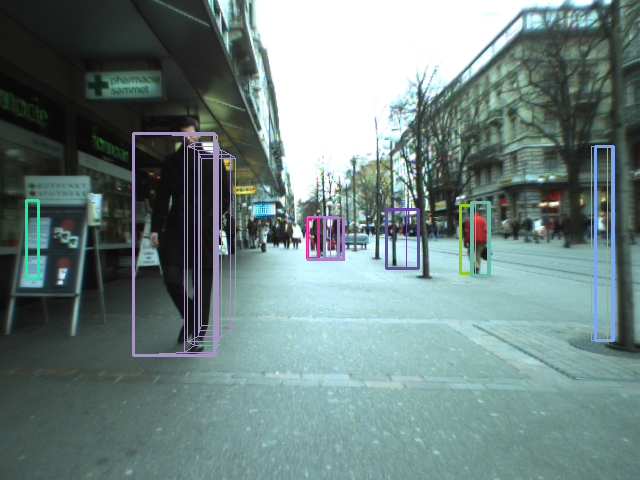
\includegraphics[width=0.45\textwidth]{sequenceTwoLevel/twolevel30}\label{fig:cp04_two_level_example_15} &
      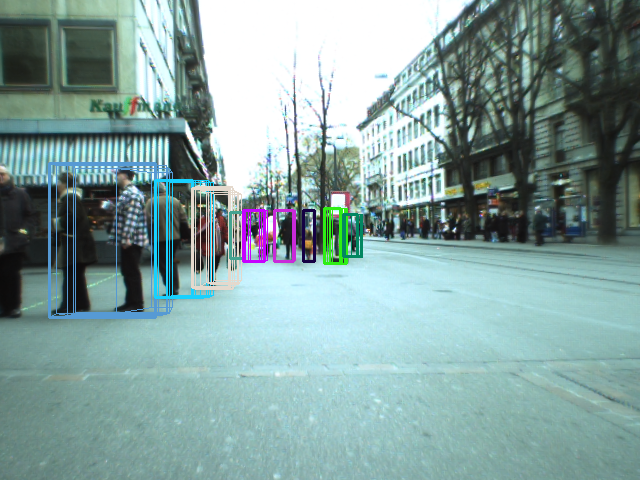
\includegraphics[width=0.45\textwidth]{sequenceTwoLevel/twolevel320}\label{fig:cp04_two_level_example_126} &
    \end{tabular}
  \caption{Some tracking results using the two-level based tracking.}\label{fig:cp04_tracking_examples_two_level}
\end{figure}

\paragraph{Object tracking case}\label{ch:chapter04_01_04_02_02}

The object tracking scheme is quite similar. However, in this case the cost matrix is not generated by counting the number of stixels associated to each obstacle, as we do not have this information (remember that for this approach, we do not apply the process described in section \ref{ch:chapter04_01_03_01}). Instead of that, we use the histograms difference for each pair of obstacles, in a process similar to that described in section \ref{ch:chapter04_01_03_01_02}, so the cost matrix in this case is defined as:

\begin{equation}\label{eq:cp04_object_matching_histograms_cost}
C(o\{t\}, o\{t - 1\}) = 1 - \left ( 2 \cdot \sqrt { 1 - \underset{i=1}{\overset{d}{\sum}}\sqrt{H(o\{t\})[i] \cdot H(o\{t - 1\})[i]}} \right )
\end{equation}

Then, the tracking problem is the same as explained for the two-level tracking case: we solve the maximization problem defined in \ref{eq:cp04_two_level_maximization}, and then the tracks are updated with the results of the matching. In figure \ref{fig:cp04_tracking_examples_object}, some other examples of the output obtained after applying this process are shown.

\begin{figure}[h!]
    \centering
    \begin{tabular}{ccccc}
      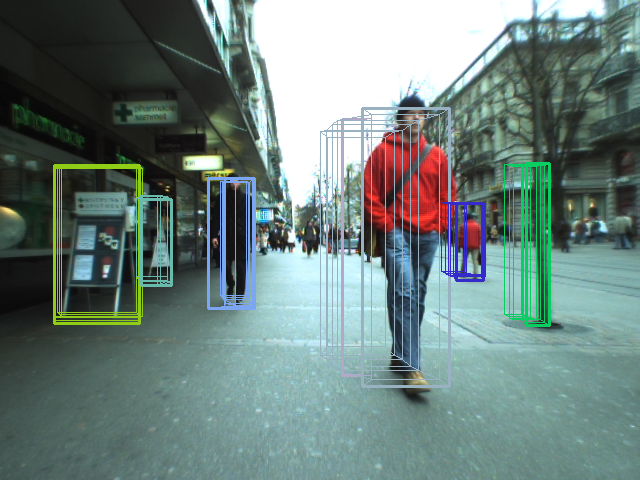
\includegraphics[width=0.45\textwidth]{sequenceObstacle/obstacle15}\label{fig:cp04_object_level_example_30} &
      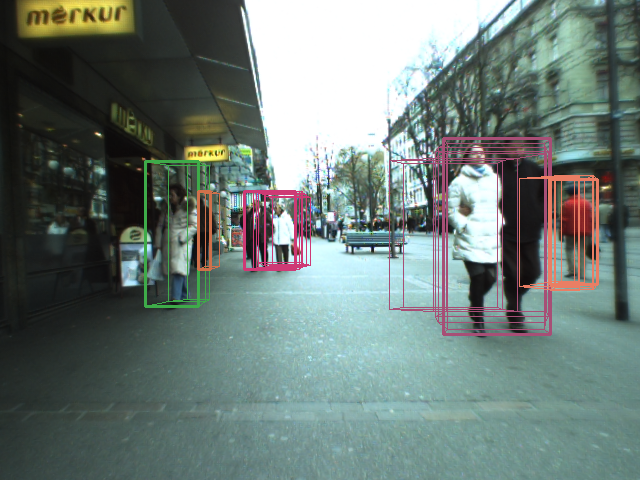
\includegraphics[width=0.45\textwidth]{sequenceObstacle/obstacle126}\label{fig:cp04_object_level_example_320}
    \end{tabular}
  \caption{Some tracking results using the object based tracking.}\label{fig:cp04_tracking_examples_object}
\end{figure}


\section{Summary}\label{ch:chapter04_07}

In this chapter, we have seen a different solution for the object tracking for driver assistance applications, based on the stixel world by \cite{badino2009stixel}. Our work extends the work presented by \cite{gunyel2012stixels}, improving the results obtained by them. The use of a two-level based tracking gives robustness to the stixel tracking and is able to improve the reconstruction by joining stixels that were not in the same plane due to a bad reconstruction. We demonstrate that using the Hellinger distance between histograms give better results than the pure Sum of Absolute Differences, and that the use of the height as matching metric is negligible.
We also saw another tracking method in which the tracking is performed at obstacle level. In this case, results were not so good, but in certain applications can be useful due to a high performance time and a low decay in the recall when the frame rate is low.
In the future, we want to try to improve the way in which stixels are computed. We think that using the polar rectification for combining tracking and reconstruction could give good results. Also, the use of a measure of the goodness of the tracks at stixel level should help to improve the results obtained for the clustering process.
In the next chapter, we will see another obstacle tracking method in which 3D dense reconstruction is used as input.

